\documentclass{article}
\usepackage[utf8]{inputenc}

\title{COMP 138 Reinforcement Learning: Programming Assignment 1}
\author{Casey Owen}

\usepackage{natbib}
\usepackage{graphicx}
\usepackage{subcaption}

\begin{document}

\maketitle

\begin{figure}[h]
\centering

\includegraphics[scale=0.125]{Slot Machines.jpg}
\caption{Slot Machines \citep{unsplash_photo_2020}}
\label{fig:slot machines}
\end{figure}

\section{Introduction}
So-called "bandit problems" represent one of the most basic forms of reinforcement learning problems. An agent is faced repeatedly with a choice of $k$ different options, and after making each choice, is presented with a numerical reward. The agent's goal is to learn which actions maximize its total reward over a given time period, and then to take those actions. A common analogy is to that of a slot machine - a person sits in front of a slot machine with many levers, and repeatedly pulls them, observes the monetary reward each time, and adjusts their strategy accordingly.

While a $k$-armed bandit problem is not yet a full reinforcement problem, which includes states, policies, and an agent capable of taking actions that change the given state, it is still a good start. This more complex version of the problem requires agents to do two important extra steps - associate a given situation (state) with the best action for the situation, and to consider the future implications of their actions. 

The $k$-armed bandit problem involves only one task - learning the best action from past results. This simplification allows us to cut out the noise and focus on this step completely, seeking strategies to optimize learning best actions. To explore this, I created a simulation of a bandit problem in a non-stationary scenario, and tested different strategies to see which would allow the agent to perform the best.

\section{Background}
We can separate the task of learning the best action into two distinct sub-parts - $\textit{action-value methods}$, which determine how an agent perceives the value of each action, and $\textit{action-selection methods}$, which determine how an agent chooses an action based on it's perceived values. Action-value methods primarily deal with the strategies for weighting recent events vs. events far in the past, and action-selection methods primarily deal with balancing exploration and exploitation.

\subsection{Action-Value Methods}
The problem examined below considers two action value methods - $\textit{sample average}$ action-selection and $\textit{constant alpha}$ action-selection. 

The sample average method is simple and perhaps the most intuitive - it values each possible action, or "arm", as the total average reward the agent has observed from that arm over the course of the simulation. However, since for extremely long simulations storing the entire reward history for every action is often intractable, an incremental update method is used instead:

$$Q_{n+1} = Q_n + \frac{1}{n}[R_n - Q_n]$$

$R_n$ and $Q_n$ represent the reward and perceived value of the action after selecting it $n$ times, where $Q_n$ is initialized as 0. This is equivalent to storing all possible rewards and taking the overall average at every step, but only requires storing two values for each action, $Q_n$ and $n$, making it much cheaper in both memory and computation.

The constant alpha method is a slight variation on the above formula. If you consider the $\frac{1}{n}$ factor to be a step-size parameter, then a more general form of the equation could be written as

$$Q_{n+1} = Q_n + \alpha[R_n - Q_n]$$
with step-size $\alpha$. Thus the sample average is a special case of the above formula, with $\alpha=\frac{1}{n}$. The constant alpha action-value method uses the same formula, but with a constant, preset value of $\alpha$ throughout the entire simulation. This allows all new points to be given the same amount of weight, no matter how many times that action has been selected before. With sample average, the contribution of each point deteriorates as the simulation runs.

\subsection{Action-Selection Methods}

Action-selection methods determine how the agent chooses an action based on its perceived values. An obvious first choice for a strategy may be to simply always pick the highest-valued action ($\textit{exploiting}$) - however, this does not consider that the agent may not have complete information about it's environment yet. The agent must first try things it is uncertain about the value of in order to gain information ($\textit{exploring}$).

${\epsilon}\textit{-greedy}$ action-selection represents a way to balance exploring and exploiting by choosing between the two randomly. $\epsilon$ is an adjustable parameter between 0 and 1 that represents the portion of time that the agent explores by choosing an action at random. All other times, the agent exploits, and chooses the action it believes to be the best.

$\textit{Upper-confidence-bound (UCB)}$ action-selection is a somewhat more complex technique for choosing actions that attempts to incorporate the uncertainty an agent has in each action's value. It does this by selecting actions according to the below formula:
$$A_t = argmax_a(Q_t(a) + c \sqrt{\frac{\ln{t}}{N_t(a)}})$$
$Q_t(a)$ is the perceived value of action $a$ at time $t$, $N_t(a)$ is the number of times that action $a$ has been selected prior to time $t$, and $c$ is a parameter controlling the degree of exploration. This formula is based on the idea of choosing the action which has the most potential to be optimal - the action with the highest upper-confidence bound in the confidence interval of action-values.
  
\section{Problem Statement}
The problem considered in this report is a special case of a bandit problem - a non-stationary bandit. That is, a bandit where the reward probability distributions change over time. In this case, the bandit considered has 10 arms, and each arm has an initial intrinsic value of 0, where the reward sampled is Gaussian with a mean of its intrinsic value and unit variance. Then, at each time step, each arm takes a random walk by incrementing its intrinsic value by a value sampled from a Gaussian distribution with mean 0 and standard deviation 0.01. The variance of each arm's reward probability function does not change.

\section{Motivation}
Examining a non-stationary problem will allow me to draw conclusions about which strategies for learning the best action are most applicable to situations with dynamic rewards functions, where the agent is forced to adapt to the new situation at every time step. These dynamic situations are often encountered in the real world since many real systems are dynamic. 

For example, in the context of a retail store, consider an agent tasked with picking from a list of products to display prominently to the customer at the entrance, where the reward function is based on sales of that product at the end of each day. It is critical that the agent be able to adjust to a changing environment where there is fluctuating demand for the various products due to seasonality and a variety of other factors.


\section{Experiment}
To model this problem, I coded simulations of the problem in Python using an object-oriented approach. I created a bandit that has non-stationary reward functions, and an agent that is capable of any of the action-value and action-selection methods described above.

In this problem, I examine all 4 possible scenarios, which represent all possible combinations of these action-value and action-selection methods, using respective parameters of $\epsilon=0.1$, $\alpha=0.1$, and $c=2$ for each method. Each simulation is 10,000 time steps long, and each scenario presents the results as the average of 2,000 simulations.

For each scenario, two metrics are calculated and plotted as a function of time - the average reward the agent receives, and the portion of simulations in which it chooses the optimal action.

\section{Hypothesis}
I believe that in all scenarios, the constant alpha action-value method will prove to be superior to sample-average over the entire simulation. By the last time steps, the bandit arms will still be continuing their random walk while the sample average method is giving increasingly tiny weight to any new results. Whereas constant alpha will be preferentially weighting recent results in the overall action-value equations.

For the action-selection methods, I believe that the $\epsilon$-greedy method will outperform UCB by the end of the simulation. I believe that UCB will suffer a similar issue, since it was designed to work on stationary problems and will struggle to adapt to a non-stationary environment. When using confidence intervals, a key assumption is that all samples were taken from the same random variable, which is not the case for non-stationary problems.

\section{Results}
\subsection{Epsilon Greedy Action-Selection}
\maketitle

\begin{figure}[ht]
% \centering

\begin{subfigure}{0.5\textwidth}
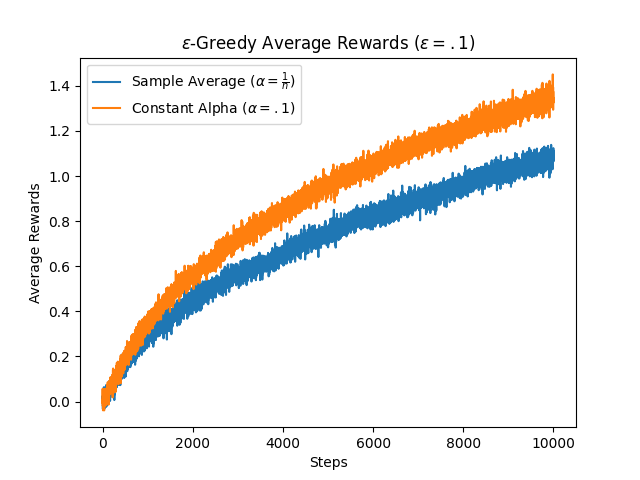
\includegraphics[scale=0.4]{epsilon_greedy_average_rewards.png} 
\caption{$\epsilon$-Greedy Average Rewards}
\label{fig:epsilon-greedy average rewards}
\end{subfigure}
\begin{subfigure}{0.5\textwidth}
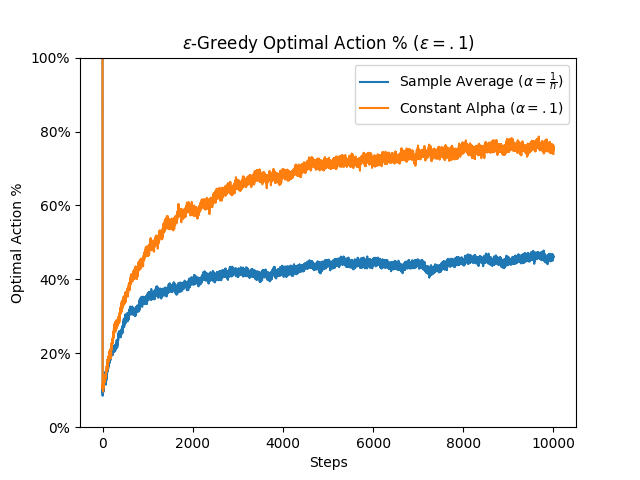
\includegraphics[scale=0.4]{epsilon_greedy_optimal_action_pct.png}
\caption{$\epsilon$-Greedy Optimal Action Percentage}
\label{fig:epsilon-greedy optimal action pct}
\end{subfigure}
\caption{$\epsilon$-Greedy Results}
\end{figure}

The results from the $\epsilon$-greedy simulations are consistent with my hypothesis - the constant alpha method is superior to the sample average method over the course of the simulation. What surprised me, however, was how early in the simulation its superiority emerged. I thought that it was possible that the sample average method would outperform in the early stages of the simulation, while all rewards were still approximately the same, but this was not the case. Since from the very first time step, all rewards are non-stationary, it is apparent that giving higher weight to the recent observations is immediately useful. 

This superiority is made clear from both the average rewards plot and the optimal action percentage plot. The constant alpha method is very clearly taking the optimal action a much higher percentage of the time, converging to about an 80\% success rate against the sample average method's 40\%. This is very impressive, since using an $\epsilon$-greedy method limits the agent to never taking the optimal action more than 91\% of the time in the 10-arm case with $\epsilon=0.1$.

I should also note the irregularity at the beginning of the optimal action percentage results - both methods have a 100\% success rate of choosing the optimal action at time step 1. This is expected, since all actions start with a reward of 0, and are thus all considered optimal. The success rate then immediately drops to 10\%, which makes sense given that there are 10 arms and the agent has no information about which is the best after one step of random walking.

Another observation of note is that the optimal action percentage graphs appear to converge to certain values, while the average rewards do not - they continue to increase after 10,000 steps. This is also expected, since one would not expect the average rewards to converge - the bandit rewards continue to change for as long as the simulation runs. However, the ultimate success rate that the strategies enjoy does not depend on the raw reward value, only their ability to adapt to new information, which does not change as the simulation runs.

\subsection{Upper-Confidence-Bound Action-Selection}
\maketitle

\begin{figure}[ht]
% \centering

\begin{subfigure}{0.5\textwidth}
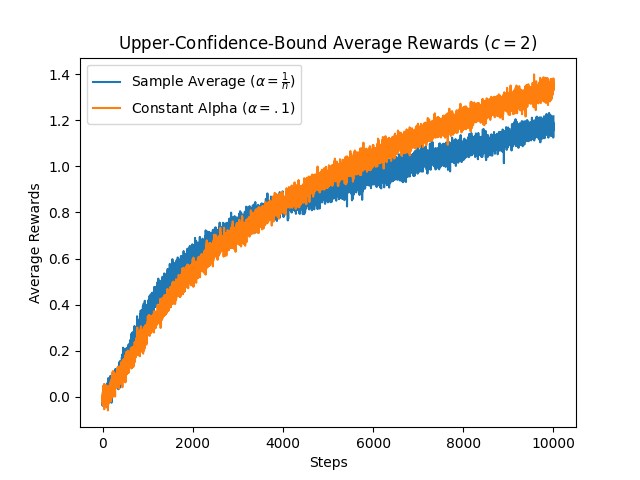
\includegraphics[scale=0.4]{ucb_average_rewards.png} 
\caption{UCB Average Rewards}
\label{fig:ucb average rewards}
\end{subfigure}
\begin{subfigure}{0.5\textwidth}
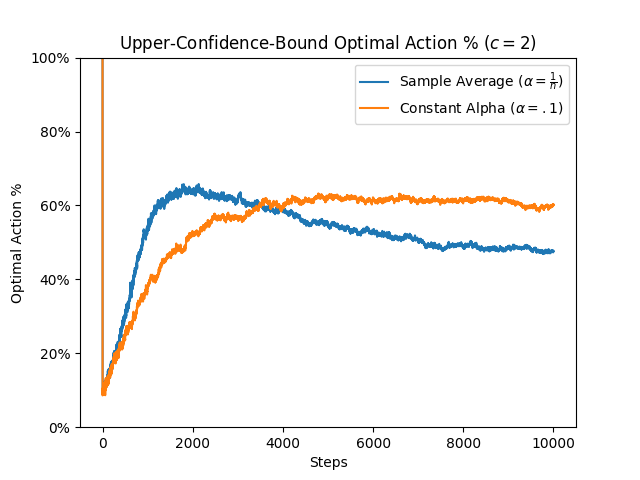
\includegraphics[scale=0.4]{ucb_optimal_action_pct.png}
\caption{UCB Optimal Action Percentage}
\label{fig:ucb optimal action pct}
\end{subfigure}
\caption{UCB Results}
\end{figure}

Once again, the constant alpha action-value method shows success is the long run, and proves able to adapt to changes more successfully than the sample average method. However, there is a key difference when using UCB action-selection, which is that for the first 4,000 time steps, the sample average method is superior.

One possible reason for this is that when using sample average and UCB at the same time results in an agent that discounts new data twice, since both methods down-weight the new contribution of evidence if it has been selected many times. This should result in an agent that is very poor at adapting to non-stationary problems. Since the arms that start out with the highest rewards early in the simulation tend to be the same arms that have the highest rewards for the first few thousand time steps, it could be that this method is using its knowledge from very early in the simulation to exploit early on. This could result in out-performance over the constant alpha method, as constant alpha is likely to explore more often.

Comparing the two action-selection methods, the results are consistent with my hypothesis that the $\epsilon$-greedy method outperforms UCB. It can be seen that the $\epsilon$-greedy method at its best reaches an 80\% success rate of choosing the optimal action by the end of the simulation, whereas the best version of UCB only reaches about 60\%. 

I believe the reason for this this matches the reasoning of my hypothesis, which is that when using UCB it is assumed that all samples were taken from the same random variable, and this was not the case in the non-stationary simulation. UCB makes the faulty assumption that if you have sampled an action many times then you are very certain of its result, even if those samples were a very long time ago and no longer match the current state.

\section{Conclusion}
The results of these simulations are useful in informing our use of action-value methods and action-selection methods for non-stationary problems. Although simulations were only ran in the simple case of the 10-armed bandit problem and are do not broadly generalize, there are still takeaways that can be applied to more complicated, realistic problems. First, that constant alpha action-value methods are much better than sample average for non-stationary problems. Second, that Upper-Confidence-Bound action-selection in the given formulation is not suited to non-stationary problems, where the rewards distributions are expected to change by a significant amount over a long period of time. Further work should be done to test these result in practice and more specifically characterize the circumstances which affect each method's performance.

\bibliographystyle{plain}
\bibliography{references}
\end{document}
